\documentclass{scrartcl}

% packages
\usepackage{amsmath}
\usepackage{amssymb}
\usepackage[ngerman]{babel}
\usepackage{booktabs}
\usepackage[font=small,labelfont=bf]{caption}
\usepackage{csquotes}
\usepackage{float}
\usepackage{fontspec}
  \setmainfont[Ligatures=TeX]{Tex Gyre Pagella}
\usepackage{graphicx}
\usepackage[pdfusetitle,unicode]{hyperref}
\usepackage{mathtools}
\usepackage{microtype}
\usepackage{siunitx}
  \sisetup{separate-uncertainty=true}
\usepackage{subcaption}
\usepackage[math-style=ISO,bold-style=ISO]{unicode-math}
  \setmathfont{Tex Gyre Pagella Math}
\usepackage{xfrac}

% options
\setlength{\parindent}{0pt}  % no stupid indentation

% commands
\DeclarePairedDelimiter{\abs}{\lvert}{\rvert}
\DeclarePairedDelimiter{\mean}{\langle}{\rangle}
\renewcommand{\vec}[1]{\mathbf{#1}}
\renewcommand{\i}{\mathrm{i}}
\DeclareRobustCommand{\e}{\ensuremath{\mathrm{e}}}

% meta
\author{Kevin Dungs \and Kevin Heinicke \and Holger Stevens}
\title{Computational Physics}
\subtitle{Übungsblatt 4}

% document
\begin{document}
\maketitle

\section*{Hausaufgabe 9: Sampling und Integration in hohen Dimensionen}
\paragraph{(a)} Das Volumen der $d$-dimensionalen Einheitskugel ist
\begin{equation}
    V_S(d) = \frac{\pi^{\sfrac{d}{2}}}{\Gamma(1 + \sfrac{d}{2})}
\end{equation}
In \autoref{fig:analytical} ist der Verlauf des Zusammenhangs für $d=1\dots200$ dargestellt.

\begin{figure}[H]
    \centering
    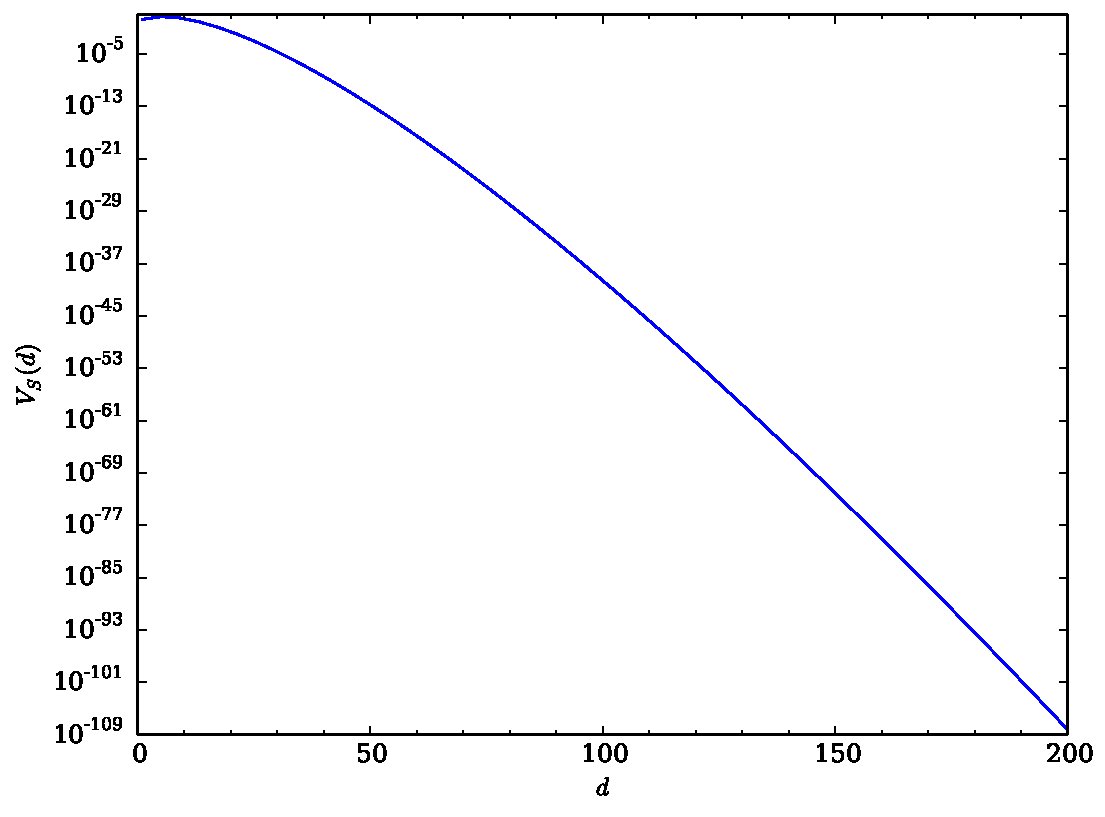
\includegraphics[width=0.5\textwidth]{plots/analytical.pdf}
    \caption{Volumen der Einheitskugel in Abhängigkeit der Dimension.}
    \label{fig:analytical}
\end{figure}

\paragraph{(b)} Das Volumen des Einheitswürfels ist unabhängig von der Dimension immer \num{1}. Das Verhältnis der beiden Volumina wird daher mit steigender Dimension immer kleiner. Für hohe Dimension würden beim Direct Sampling also quasi alle Würfe verworfen und es ließen sich nur mit sehr sehr vielen Durchläufen Ergebnisse erzielen.

\paragraph{(c)} Die Funktion \texttt{MCMC\_X2} in \texttt{mcmc\_volume.cc} approximiert $\mean{x^2}$ für gegebene Dimension und Anzahl Schritte. Die Funktion gibt ein \texttt{std::tuple} mit zwei Einträgen, dem Mittelwert und dem Fehler des Mittelwerts, zurück. Ein Testlauf für $d=2$ ergibt $\mean{x^2} = \num{0.500411 \pm 0.000288}$. Auch bei mehreren Durchläufen ist der Wert immer auf drei Nachkommastellen genau.

\paragraph{(d)} Nach der verwendeten Vorschrift ergibt sich für das Volumen $V_C(d+1)$ des $d+1$-dimensionalen Einheitszylinders

\begin{equation} \label{eq:VC}
    V_C(d+1) = 2 V_S(d)
\end{equation}

Die Größe $\mean{Q}$ ist das Verhältnis der Volumina von $d+1$-dimensionaler Einheitskugel und $d+1$-dimensionalem Einheitszylinder. Es ist also

\begin{equation*}
    \mean{Q} = \frac{V_S(d+1)}{V_C(d+1)} \overset{\eqref{eq:VC}}{=} \frac{V_S(d+1)}{2 V_S(d)} \tag*{\square}
\end{equation*}

Die Funktion \texttt{MCMC\_Q} in \texttt{mcmc\_volume.cc} approximiert $\mean{Q}$ analog zu $\mean{x^2}$ in Teil (c). Die Mittelwerte und Fehler werden für $d = 1\dots199$ in einer Textdatei gespeichert. Das Pythonscript \texttt{plot.py} ließt die Werte ein und berechnet daraus $V_S$. In \autoref{fig:mcmc} ist der Verlauf der analytisch berechneten und der mit MCMC approximierten Werte dargestellt. Außerdem sind die Pulls\footnote{Absolute Abweichung normiert auf Fehler} abgebildet. Es ist

\begin{align*}
    V_{S}(200) &= \num{5.5588328420278045e-109} \\
    V_{S,\text{MCMC}}(200) &= \num{6.1 \pm 0.7e-109} \\
    \text{pull} &= \num{0.76}\,\sigma
\end{align*}

\begin{figure}[H]
    \centering
    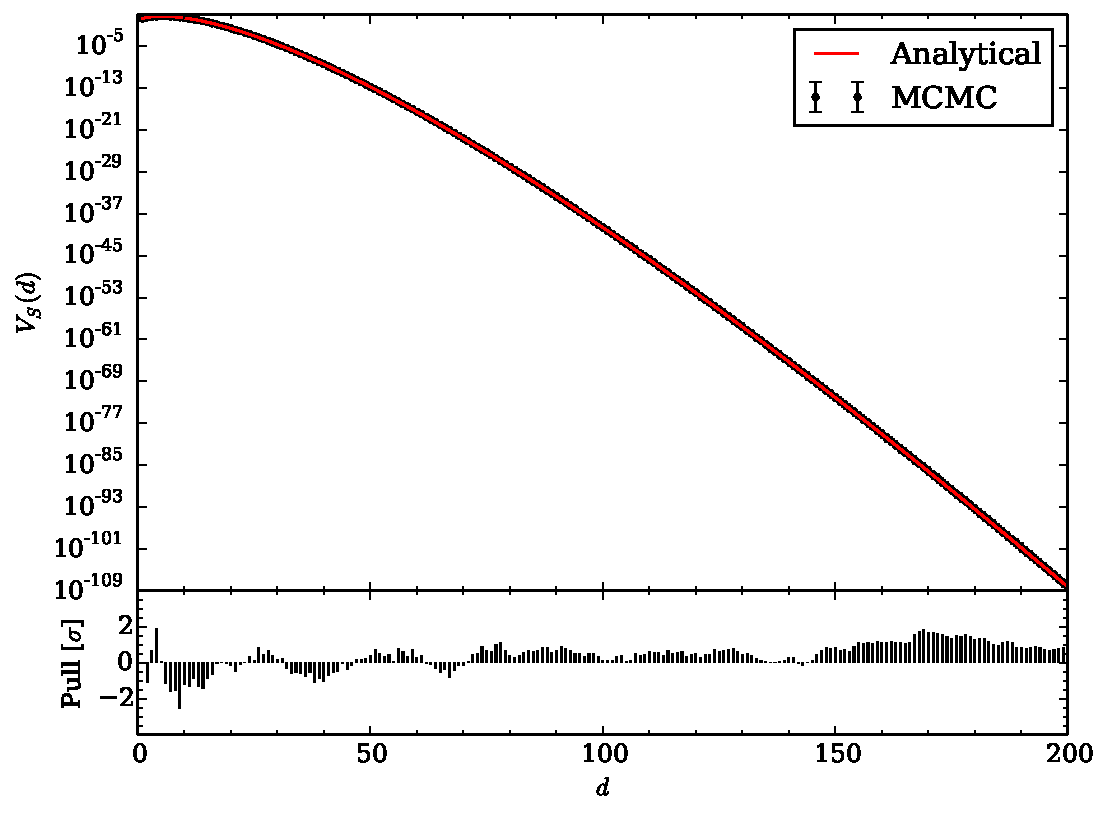
\includegraphics[width=0.9\textwidth]{plots/plot.pdf}
    \caption{Volumen der Einheitskugel in Abhängigkeit der Dimension mit MCMC. Die Pullverteilung legt nahe, dass das MCMC die Werte hier \emph{eher} über- als unterschätzt.}
    \label{fig:mcmc}
\end{figure}

\end{document}
